\section{Procedure}
%In this section we present the procedure that was followed to trap a polaron in rutile. We start with a standard calculation on a rutile unit cell, followed by a DFT+U calculation. Then, we trap an extra electron in a supercell, and we compute the properties of the polaron investigating the DOS and band structure. The calculation of a delocalized electron is discussed as well, and the two solutions are compared.
\subsection{DFT and DFT+U calculation on rutile}
We began by performing a standard DFT calculation on rutile. To do so, we first needed some information on the material we were investigating. Rutile has a tetragonal unit cell, with two titanium and four oxygen atoms inside. A sketch of the unit cell is shown in \cref{fig:rutile}.
\begin{figure}
    \centering
    \begin{subfigure}[t]{0.48\textwidth}
        \centering
        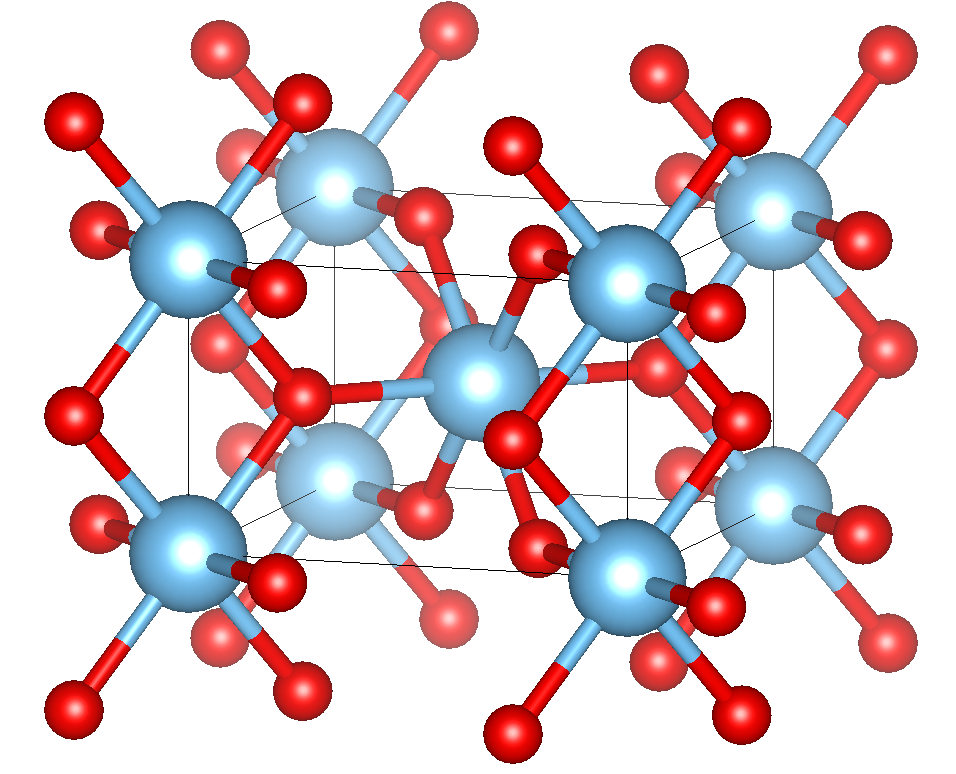
\includegraphics[width=1\textwidth]{figures/rutile.png}
        \caption{Unit cell}
        \label{fig:rutile}
    \end{subfigure}
    \hfill
    \begin{subfigure}[t]{0.48\textwidth}
        \centering
        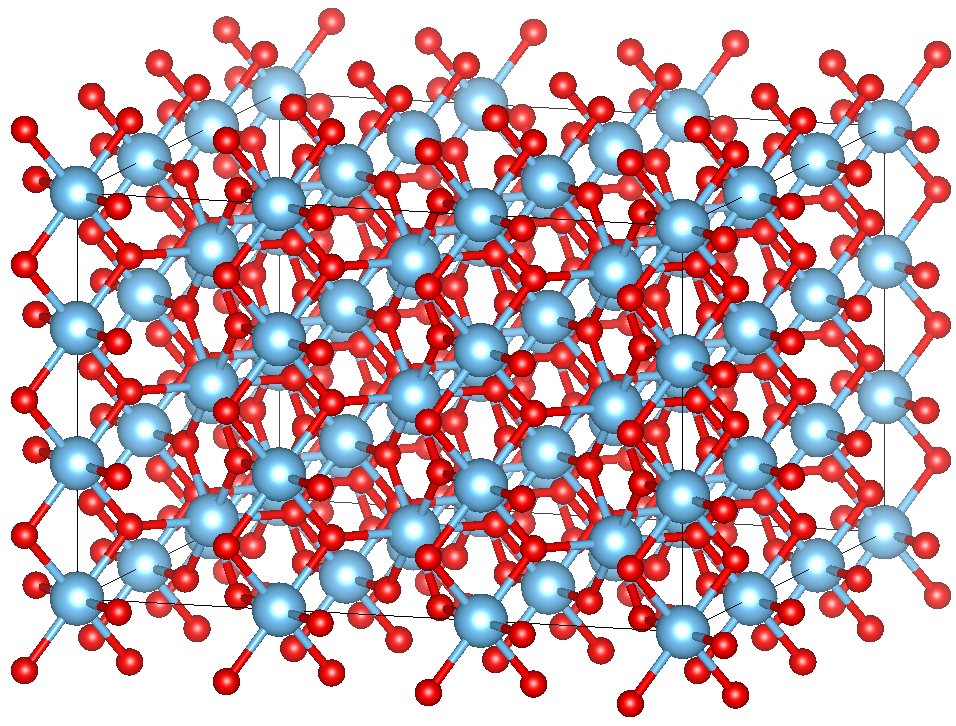
\includegraphics[width=1\textwidth]{figures/supercell.png}
        \caption{$3\times3\times3$ supercell}
        \label{fig:supercell}
    \end{subfigure}
    \caption[Rutile unit cell and supercell]{Rutile unit cell and supercell. Titanium is blue and oxygen is red. The images have been rendered with Vesta \cite{zotero-174}.}
\end{figure}
The lattice parameters and the positions of the atoms were taken from The Materials Project website \cite{osti_1184648} and inserted in the  POSCAR file. The properties of the atoms, as discussed in \cref{sec:implementation}, are described by  pseudopotentials. For titanium atoms, a projector augmented wave (PAW) pseudopotential with 12 valence electrons ($3s^2 3p^6 4s^1 3d^3$) was used, whereas for oxygen atoms a PAW pseudopotential with 6 valence electrons ($2s^2 2p^4$) was chosen. For the k-points grid, we used a $7\times7\times11$ $\Gamma$-centered grid, with a spacing of about \SI{0.03}{\angstrom^{-1}}.

With these settings, a series of DFT calculations was performed. In all the calculations we set the cut-off energy to \SI{700}{eV}. The convergence process was stopped when both the energy difference between two successive electronic calculations was smaller than $10^{-8}$~\SI{}{eV} and the forces acting on the ions were smaller than \SI{0.01}{eV/\angstrom}. A Gaussian smearing of $\sigma = 0.05$ was used for the calculations that involved the relaxation of the lattice or the computation of the band structure. On the other hand, for the computation of the density of states (DOS), the tetrahedron smearing method was used. The tetrahedron method usually gives better results, but VASP does not implement it for calculations where the position of the ions changes.% or where the k-points grid is not uniform.

Before investigating the electronic properties of the material, we wanted to be sure that the structure was properly relaxed. A non-spin-polarized calculation was performed on the unit cell in order to allow the relaxation of the ions positions. The volume and the shape of the unit cell was kept constant, allowing the atomic positions to change. This was achieved by performing a series of standard electronic DFT calculations. When electronic convergence is reached, the forces acting on the ions are computed, and the ions positions are updated minimizing the forces. Then, another electronic calculation is run. The process is stopped when both the electronic and the ionic calculations converge.

The relaxed structure was employed in a standard self-consistent DFT calculation. In particular, the DOS, the electronic charge density and the wavefunctions were computed. The result was used in a non-selfconsistent calculation to compute the band structure. The bands were calculated along a special path of k-points. Conventionally, these points are named  $\Gamma$-X-M-$\Gamma$-Z-R-A-Z; X-R; M-A, and they are high-symmetry points of the first Brillouin zone of a tetragonal system. The positions of these points in the Brillouin zone are shown in \cref{fig:symmetry_points}. The path was created connecting each couple of high-symmetry k-points with a line of 10 evenly-spaced points.

\begin{figure}
    \centering
    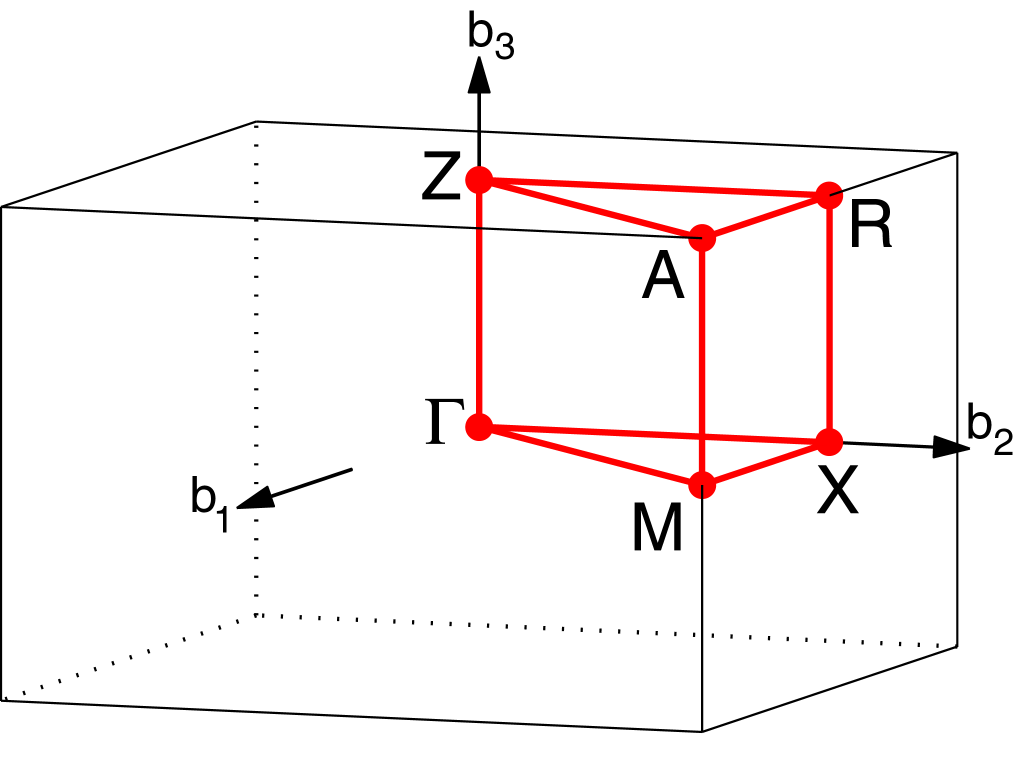
\includegraphics[width=0.5\textwidth]{figures/brillouin_zone}
    \caption[Brillouin zone of a tetragonal system]{Brillouin zone of a tetragonal system, the red path passes through the high-symmetry points of the zone. $\vec{b}_1, \vec{b}_2, \vec{b}_3$ are the reciprocal basis vectors of a tetragonal unit cell. The path used in the calculation of the band structure was $\Gamma$-X-M-$\Gamma$-Z-R-A-Z; X-R; M-A.}
    \label{fig:symmetry_points}
\end{figure}

As discussed in \cref{sec:dft+u}, DFT often fails to give appropriate results in band-gap calculations. To avoid the problem, the previous calculations were repeated in DFT+U.  The DFT+U correction was implemented following the Duradev approach, setting the value of $U-J$ to \SI{3.9}{eV}. This value was determined by Reticcioli et al. entirely from first principles \cite{reticcioli2022}, using the constrained random phase approximation (cRPA) \cite{aryasetiawan2006}. The correction was applied to the titanium d-orbitals, leaving the other orbitals unaltered. In fact, as discussed in \cref{sec:dft+u}, s- and p-orbitals are less localized than d-orbitals, and they do not need corrections. Starting with the relaxed structure, we relaxed it again with the DFT+U correction. The DOS and band structure were computed as well, following the same procedure that was described above.

\subsection{Electron localization}
To find a polaronic solution, we had to add an extra electron to the system and localize it at the centre of the cell. Since the electron had to be localized in a region comparable with the size of a unit cell, the simulation could not be run on a unit cell alone. VASP, as many other DFT software packages, uses periodic boundary conditions, so the electron would interfere with itself at the cell boundaries. A large-enough supercell is needed to avoid self-interaction errors. For this reason, large polarons are hard to simulate in DFT: the supercell size  makes the calculation computationally very expensive.

A $3\times3\times3$ supercell was created repeating the relaxed unit cell three times in each direction. The unit cell that was repeated was the result of the relaxation performed with the DTF+U correction. A sketch of the supercell is shown in \cref{fig:supercell}. Given the bigger size of the cell, to have $k$-points separated by \SI{0.03}{\angstrom^{-1}}, a $2\times2\times4$ grid was enough. The usual calculations described above were performed on the supercell, computing the DOS and the band structure.

Since the formation of the polaron is only slightly energetically favoured compared to a delocalized solution, the extra electron was difficult to localize. Adding one electron to the system does not result in a localized state, but in an electron delocalized in the whole supercell. To find a localized solution, a more gradual approach was necessary.

The central titanium atom was substituted with vanadium, which is the element following titanium in the periodic table. Given its higher atomic number, it has one more electron and a stronger nuclear attraction. The position of the new atom was set in the POSCAR file, and a vanadium PAW pseudopotential with 13 valence electrons ($3s^2 3p^6 4s^1 3d^4$) was added to the POTCAR file. Added the electron, a number of expedients was needed to ensure its localization. The aim was to localize it on the central atom, the vanadium one. The six oxygen atoms around the central atom were moved outwards by \SI{0.04}{\angstrom}, creating a potential well for the electron. The distortion of the lattice broke the symmetry of the system, and since VASP usually takes advantage of the symmetry of the system to fasten calculations, this feature was disabled. The $U-J$ value was set to \SI{3.9}{eV} for the titanium d-orbitals and to \SI{9}{eV} for the vanadium d-orbitals. Together, the stronger nuclear attraction, the displacement of the oxygen atoms, and the high $U-J$ value, favoured the electron localization on the central atom.

A DFT+U calculation with lattice relaxation was run.  Since the extra electron introduced a spin magnetic moment to the system, the calculation was spin-polarized. The magnetic moment was initially set to zero for every atom except for the vanadium one, for which it was set to $+\mu_B$, where $\mu_B$ is the Bohr magneton. To check if the electron localization was successful, the magnetic moments of the atoms were inspected. For a localized state, we expected the central vanadium atom to be the only one with a magnetic moment of the order of $\mu_B$. On the other hand, for a delocalized state, we expected the extra magnetic moment introduced by the additional electron to be spread on all the atoms of the supercell.

The localized solution was used to initialize a new set of calculations. The goal was to gradually substitute the vanadium atom with a high $U-J$ value with a titanium atom with a normal $U-J$ value. This was done in two steps.

Firstly, vanadium was removed and titanium was placed back, leaving the $U-J$ value applied to the central atom to \SI{9}{eV}. The number of electrons was manually set to the same number of the calculation with vanadium. The atomic positions were initialized as in the previous calculations, with the oxygen atoms shifted by \SI{0.04}{\angstrom}. The calculation was started with the charge density and wavefunctions obtained with vanadium, where the additional electron was already localized.
The calculation was spin-polarized, and the initial magnetic moment was read from the charge density file. The localization of the extra electron was checked looking at the magnetic moment of the atoms as explained above. The eigenvalues and DOS were also inspected to see if a new state was present in the middle of the band gap.

Secondly, the calculation of the polaron was done continuing the last calculation with a $U-J$ value of \SI{3.9}{eV}. The calculation was initialized with the atomic positions, charge density and wavefunctions of the previous calculation. The magnetic moments, DOS and eigenvalues were inspected again to check if the polaron was present.

\subsection{Polaron}
Different calculations were run to compute some of the polaron properties. A static electronic calculation was run starting from the previous result to compute a more precise DOS. The band structure of the polaronic solution was also computed with a non-self-consistent calculation on the usual path of k-points. Finally, the isosurfaces of the polaron charge density were computed. To do so, the charge density was decomposed over the different bands, and the contribution of the polaron was selected restricting the energy to an appropriate interval. The final result was rendered with Vesta, and the electron localization observed.

A delocalized solution was computed as well for comparison. To achieve this, an extra electron was added to the supercell and a non-spin-polarized DFT+U calculation was performed. The extra electron was added manually, setting the number of electrons to the number of the electrons in the original rutile supercell plus one. The DOS and band structure were computed and compared with the polaronic solution.